\documentclass[10pt,a4paper]{article}
\usepackage[utf8]{inputenc}

% Define the page margin
\usepackage[margin=3cm]{geometry}

% Better typography (font rendering)
\usepackage{microtype}

% Math environments and macros
\usepackage{amsmath}
\usepackage{amsfonts}
\usepackage{amssymb}
\usepackage{amsthm}

% Define \includegraphics to include graphics
\usepackage{graphicx}

% Draw graphics from a text description
\usepackage{tikz}

% Syntax highlighting
\usepackage{minted}

% Set global minted options
\setminted{linenos, autogobble, frame=lines, framesep=2mm}

% Import the comment environment for orgtbl-mode
\usepackage{comment}

% Do not indent paragraphs
\usepackage{parskip}

\title{Automata and Formal Languages, Sheet 1}
\author{Marten Lienen (03670270)}

\begin{document}

\maketitle

\section*{Exercise 1.1}

\subsection*{Part a)}

\begin{figure}[h]
  \centering
  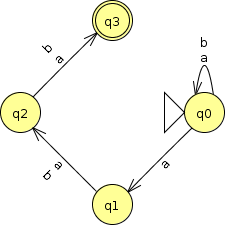
\includegraphics[width=0.5\textwidth]{sheet-1/exercise-1-a-nfa}
  \caption{NFA for 1a)}
\end{figure}

\begin{figure}[h]
  \centering
  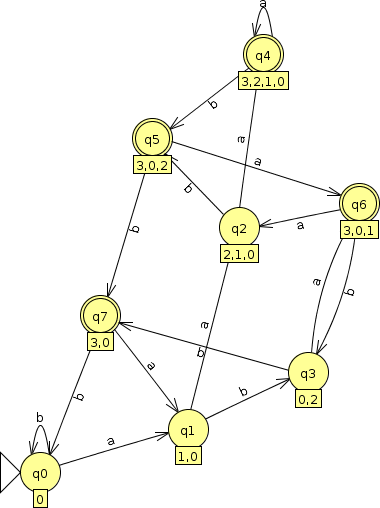
\includegraphics[width=0.5\textwidth]{sheet-1/exercise-1-a-dfa}
  \caption{DFA for 1a)}
\end{figure}

\subsection*{Part b)}

The DFA has to remember if there was an $a$ among the last $n$ read characters.
So you need at least $n + 1$ states.
One initial, non-final state $x$ that the automaton also transitions to after not having read an $a$ for $n$ transitions.
Additionally there are $n$ states, whereas state $i$ means that the last $a$ was read $i$ positions ago.
These $n$ states are all final.

\subsection*{Part c)}

\begin{figure}[h]
  \centering
  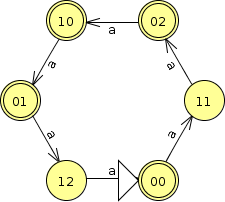
\includegraphics[width=0.5\textwidth]{sheet-1/exercise-1-c}
  \caption{DFA for $L_{3}$}
\end{figure}

\subsection*{Part d)}

The automaton is already deterministic and has $6$ states.

\subsection*{Part e)}

\begin{proof}
  It suffices to show that $L_{n}$ has at least $n(n - 1)$ different residuals.
  These are the residuals of $a^{0}, \dots, a^{n(n - 1) - 1}$.
  \begin{equation*}
    L^{a^{k}} = \{ a^{j} \in \Sigma^{*} \mid k + j \text{ is divisible by $n$ or $n - 1$} \}
  \end{equation*}
  Let $p \in [0, \dots, n(n - 1) - 2]$ and $q \in [1, \dots, n(n - 1) - p - 1]$.
  We have to show that there is an $r \in \mathbb{N}$ such that either $a^{r} \in L^{a^{p}}$ or $a^{r} \in L^{a^{p + q}}$ but not both.
  If $q$ is not divisible by $n$ nor by $n - 1$, let $r = n(n - 1) - p$.
  Then $p + r = n(n - 1)$ is divisible by $n - 1$ but $p + q + r$ is neither divisible by $n$ nor by $n - 1$ because $q$ is not.

  If $q$ is divisible by $n$ but not $n - 1$, let $r = (n + 1)(n - 1) - p$.
  Then $p + r = (n + 1)(n - 1)$ which is divisible by $n - 1$ but $p + q + r$ is neither divisible by $n$ nor by $n - 1$ because $q$ is not divisible by $n - 1$ and $p + r$ is not divisible by $n$.

  If $q$ is divisible by $n - 1$ but not $n$, let $r = n(n + 1) - p$.
  Then $p + r = n(n + 1)$ is divisible by $n$ but $p + q + r$ is not divisible by $n$ because $q$ is not divisible by $n$, neither is $p + q + r$ divisible by $n - 1$ because $p + r$ is not divisible by $n - 1$.

  $q$ cannot be divisible by both, because $n$ and $n - 1$ are relatively prime which means that their least common multiple is $n(n - 1)$ which is outside the range of $q$.
\end{proof}

\section*{Exercise 1.2}

The game has some bugs and a weird regex grammar.
I finished the levels as far as I could.

\section*{Exercise 1.3}

\subsection*{Part a)}

\subsubsection*{Regex}

\begin{align*}
  A & = aA + bB + e = aA + b(aA + e) + e = aA + baA + b + e\\
  & = (a + ba)A + b + e = (a + ba)* (b + e)\\
  B & = aA + bC + e = aA + be + e = aA + e\\
  C & = (a + b)C = (a + b)*e = e
\end{align*}

The regex is $(a + ba)* (b + e)$.

\subsubsection*{NFA-$\epsilon$}

\begin{figure}[h]
  \centering
  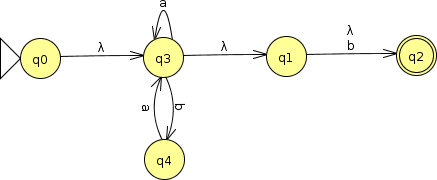
\includegraphics[width=0.5\textwidth]{sheet-1/exercise-3-a-nfa-e}
  \caption{NFA with $\epsilon$-transitions}
\end{figure}

\subsubsection*{NFA}

\begin{figure}[h]
  \centering
  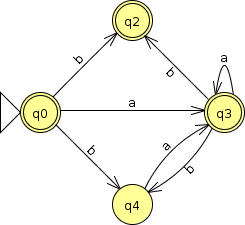
\includegraphics[width=0.5\textwidth]{sheet-1/exercise-3-a-nfa}
  \caption{NFA without $\epsilon$-transitions}
\end{figure}

\subsubsection*{DFA}

\begin{figure}[h]
  \centering
  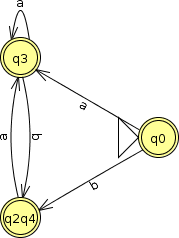
\includegraphics[width=0.5\textwidth]{sheet-1/exercise-3-a-dfa}
  \caption{DFA again}
\end{figure}

\subsection*{Part b)}

The JFLAP generated automaton in figure \ref{fig:exercise-3-b} has one more state.

\begin{figure}[h]
  \centering
  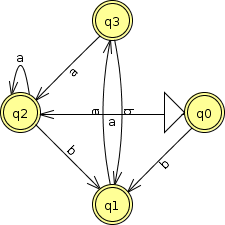
\includegraphics[width=0.5\textwidth]{sheet-1/exercise-3-b}
  \caption{JFLAP generated automaton}
  \label{fig:exercise-3-b}
\end{figure}

\subsection*{Part c)}

They are equivalent.

\section*{Exercise 1.4}

\begin{proof}
  Since $L_{1}$ and $L_{2}$ are regular, there are DFAs $A = (Q_{A}, \Sigma, \delta_{A}, q_{A0}, F_{A})$ and $B = (Q_{B}, \Sigma, \delta_{B}, q_{B0}, F_{B})$ accepting them.
  Define a new DFA $C = (Q_{C}, \Sigma, \delta_{C}, q_{C0}, F_{C})$ that informally runs $A$ on the odd positions and $B$ on the even ones.
  \begin{itemize}
  \item $Q_{C} = \{ (q_{A}, q_{B})_{A} \mid q_{A} \in Q_{A}, q_{B} \in Q_{B} \} \cup \{ (q_{A}, q_{B})_{B} \mid q_{A} \in Q_{A}, q_{B} \in Q_{B} \}$
  \item $\delta_{C} = \{ ((q_{A}, q_{B})_{A}, a, (q_{A}', q_{B})_{B}) \mid (q_{A}, a, q_{A}') \in \delta_{A}, q_{B} \in Q_{B} \} \cup \{ ((q_{A}, q_{B})_{B}, a, (q_{A}, q_{B}')_{A}) \mid q_{A} \in Q_{A}, (q_{B}, a, q_{B}') \in \delta_{B} \}$
  \item $q_{C0} = (q_{A0}, q_{B0})_{A}$
  \item $F_{C} = \{ (q_{A}, q_{B})_{B} \mid q_{A} \in F_{A}, q_{B} \in F_{B} \}$
  \end{itemize}
  Obviously $C$ accepts $S(L_{1}, L_{2})$.
\end{proof}

\end{document}
